%\let\textcircled=\pgftextcircled
\chapter{Software engineering consideration}
\label{chap:software_engineering_consideration}

This chapters deals with software engineering (SWE) topics: software design, quality measure and process management. \\
During SWE course I followed was focused on object oriented software design, that doesn't really fit for this project. The domain doesn't contain many objects to model and python classes introduce an overhead which is incompatible with performance required, taking into account input dimensions. \\
Anyway, even if I used a more functional approach, I still divided the codebase into modules using \textit{responsibility-driven design}.

\section{Requirements}
After several discussions with my supervisor, I modeled the following functional requirements:
\begin{enumerate}
\item the software will support inputs in the format specified in the \hyperref[chap:intro]{introduction chapter};
\item the software will use Blender API to animate a vehicle so that its linear and angular positions reflect the one from which the input data is measured;
\end{enumerate}
Non functional requirements are:
\begin{enumerate} 
\item \underline{performance}: the software must at least elaborate a dataset of 100.000 records in less than five minutes;
\item \underline{user experience}: the software must be easy to use also from a 3D artist point of view;
\item \underline{operating systems}. the software must support of Windows and GNU/Linux ;
\end{enumerate}

\section{Structure}
Satisfying functional requirement 1 is the main challenge of the project. Recreating a perfect reconstruction is very hard and requires many techniques as showed in the previous chapter. \\
Following the methods previously illustrated the \textit{responsibilities} of the software are:
\begin{enumerate}
\item input loading;
\item input parsing;
\item input format auto-detection;
\item noise reduction;
\item gyroscope offset drift reduction;
\item correction of vertical bad alignment;
\item correction of vertical bad alignment;
\item derivation of GNSS speed and acceleration;
\item moving from local to laboratory reference frame;
\item moving from laboratory to world reference frame;
\item integrate accelerations;
\item integrate velocities;
\item timestamps normalization;
\item dependencies auto-installation;
\item blender user-interface handling;
\item creation of animation in Blender;
\end{enumerate}

\begin{figure}[H]
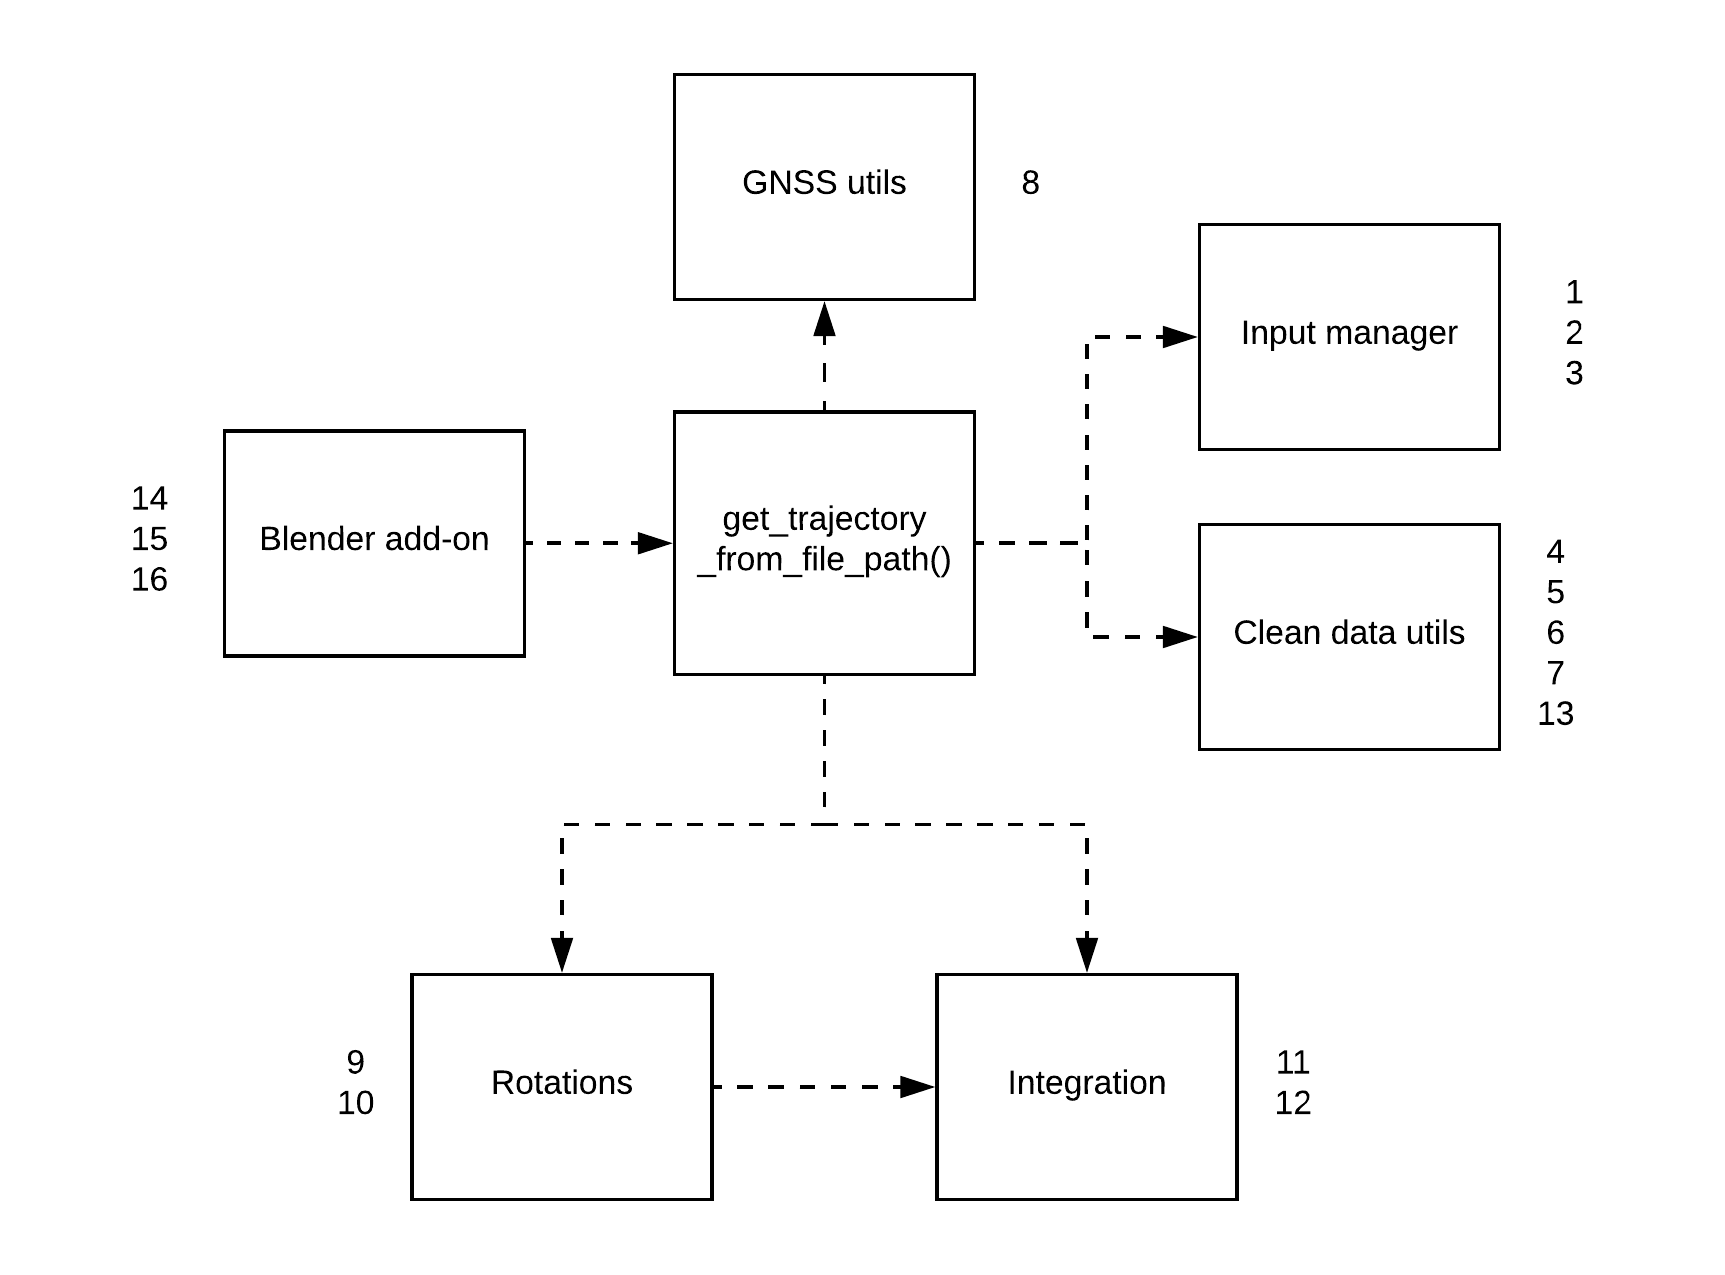
\includegraphics[width=\textwidth]{structure.png}
\caption{UML diagram showing project modules and their dependencies. The numbers nears each modules states responsabilities assigned to it.}
\end{figure}

\section{Dependency management}
Current software development practices suggest to \textit{don't reinvent the wheel} and re-use as much as existing software as possible.
Project stability is related to its dependencies' stability. Delegating responsibilities to other trusted programmers reduce project risks and increase overall quality. Specifying explicitly project dependencies is useful both for the programmer and for the user, in particular specifying which version of each dependency the software is assured to work. Python has various tools to handle this, the most popular are \textit{pip+virtualenv} and \textit{Conda}. \\
\textit{Virtual environments} allow to isolate Python packages on which the project depends on from the global system ones. This allows to use different packages version. \\
\textit{Pip} (Pip Install Packages) can install packages from a the PyPi repository, the largest one containing more than 143 hundred packages, parsing a list file containting dependencies. \\
\textit{Conda} is a package manager designed for every language, instead virtualenv is only for Python. It was created from the PyData community to overcome Pip limitations and doesn't use only PyPi to retrieve packages. Instead it has customized version of python scientific packages like numpy, scipy and pandas, optimized for performance as Conda can work on a lower-level in target machine. \\
Initially, I was using Conda and I noticed a better performance, but when I created the Blender add-on code part that auto install dependencies I had to move back to virtualenv+pip because it was easier to install.
% TODO talk about difference i found respect to virtualenv+pip and put some references

\section{Unit testing}
On the project I applied the principles of \textit{unit testing}. I tried to create a test for every function I've written, sometimes even before the code itself to be tested, to make it minimal. \\
During this process I prepared a tool to produce syntetich trajectories, to overcome specific requirements of some tests.
The tests I've written are incremental, some verify only small functionalities, others verify more overall features that use the small functionalities underneath. For example, I created a test with a complex trajectory similar to the one of a spring, to test integrator precision, then I created a circular trajectory, where body also rotate like a car in a roundabout to test, angular position integration and body rotation.
In this way it is easier when a breaking change is introduced to debug and fix the problem.\\
Right now the test coverage, which is the percentage of code lines that are executed by automatic tests, of project's principal modules is 86\%. \\ 